\section{Matrix Class Reference}
\label{classMatrix}\index{Matrix@{Matrix}}
{\tt \#include $<$matrix.h$>$}

Collaboration diagram for Matrix:\begin{figure}[H]
\begin{center}
\leavevmode
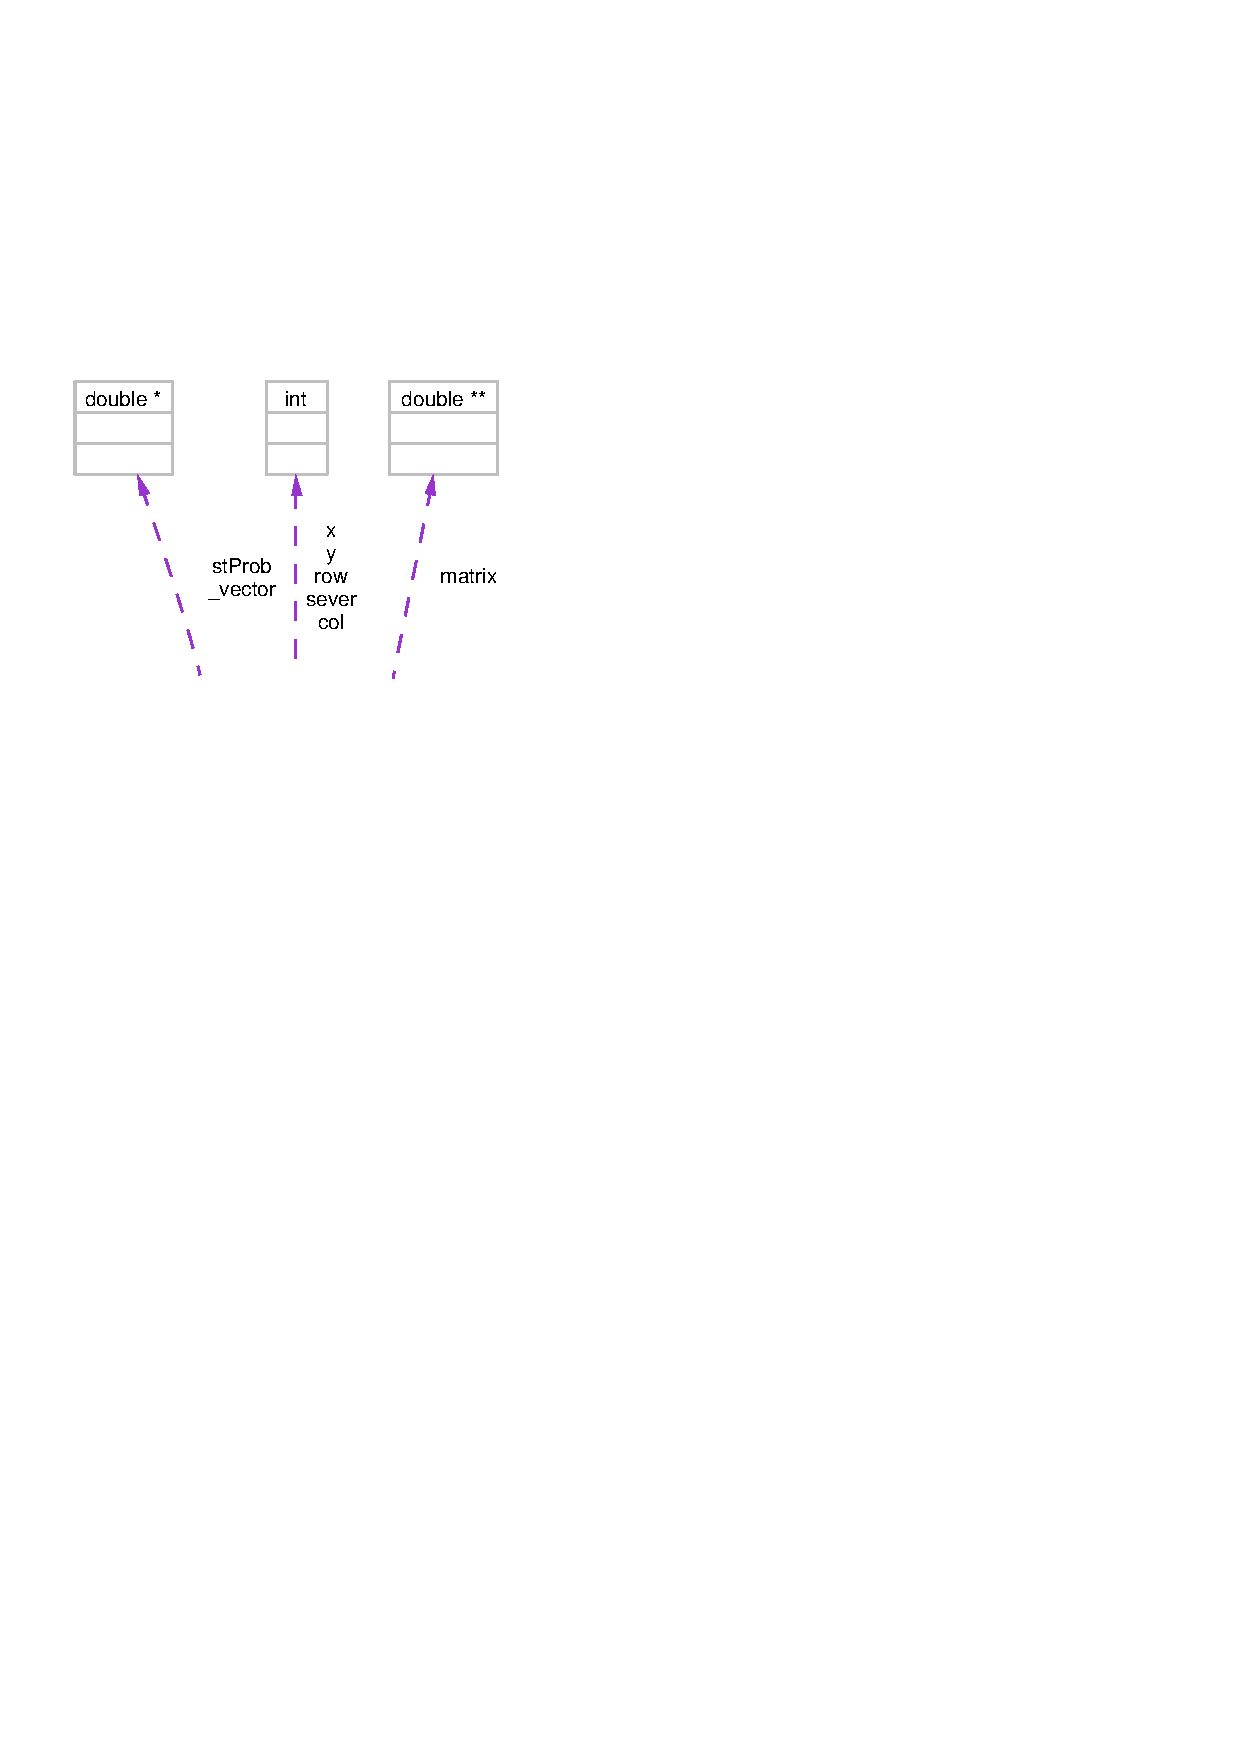
\includegraphics[width=128pt]{classMatrix__coll__graph}
\end{center}
\end{figure}
\subsection*{Public Member Functions}
\begin{CompactItemize}
\item 
{\bf Matrix} (int {\bf x}=5, int {\bf y}=5, double init=0.0)
\item 
{\bf Matrix} (const  {\bf Matrix} \&orig\-Matrix)
\item 
{\bf $\sim$Matrix} ()
\item 
{\bf Matrix} \& {\bf operator=} ({\bf Matrix} \&m)
\item 
double {\bf operator()} (int a, int b)
\item 
void {\bf Include\-Array} (double array[$\,$], int from, int to)
\item 
void {\bf Get\-Vector} (char $\ast${\bf file\-Name})
\item 
void {\bf Get\-Vector} (vector$<$ float $>$ new\-Vector)
\item 
void {\bf Include\-Vector} ()
\item 
void {\bf Adjust\-Vector} (int, int, int, int)
\item 
void {\bf Adjust\-Matrix} (int, int, int, int, int, int)
\item 
void {\bf Build\-Matrix} (double[$\,$])
\item 
void {\bf Build\-Matrix2} ({\bf List}$<$ int $>$ \&, int)
\item 
void {\bf Trim\-Matrix} (int type, float density, int remain0, int dur\-Loc)
\item 
void {\bf Choose\-M} ()
\item 
void {\bf Choose\-M} (int \&r, int \&c)
\item 
void {\bf Envelopes} (char $\ast${\bf file\-Name})
\item 
void {\bf Envelopes} (vector$<$ float $>$ probs, vector$<$ Envelope $\ast$ $>$ env\-List)
\item 
void {\bf Envelopes} (vector$<$ float $>$ probs, vector$<$ int $>$ env\-Nums, vector$<$ float $>$ coeffs)
\item 
void {\bf Envelopes} (char $\ast${\bf file\-Name}, vector$<$ Collection$<$ xy\_\-point $>$ $>$ xy\-Collection, vector$<$ vector$<$ string $>$ $>$ segment\-Types, vector$<$ vector$<$ string $>$ $>$ segment\-Fixed)
\item 
void {\bf Envelopes} (vector$<$ Collection$<$ xy\_\-point $>$ $>$ xy\-Collection, vector$<$ vector$<$ string $>$ $>$ segment\-Types, vector$<$ vector$<$ string $>$ $>$ segment\-Fixed)
\item 
void {\bf Interpol} (int, double[$\,$])
\item 
void {\bf Mult} (int remain0, float density, int type, int dur\-Loc, int dur\-Array[$\,$], int stime\-Matrix, int star\-Tarray[$\,$])
\item 
void {\bf Normalize} ()
\item 
void {\bf Set\-Dim} (int {\bf x}, int {\bf y})
\item 
double {\bf Get\-Value\-At} (int {\bf x}, int {\bf y})
\item 
void {\bf Init} (double init)
\item 
void {\bf Print} ()
\item 
void {\bf Print\-Vector} ()
\item 
void {\bf Clear} ()
\item 
int {\bf Get\-X} ()
\item 
int {\bf Get\-Y} ()
\end{CompactItemize}
\subsection*{Public Attributes}
\begin{CompactItemize}
\item 
int {\bf col}
\item 
int {\bf row}
\item 
double $\ast$$\ast$ {\bf matrix}
\end{CompactItemize}
\subsection*{Private Member Functions}
\begin{CompactItemize}
\item 
void {\bf Smooth} (int, int, int, int, int)
\end{CompactItemize}
\subsection*{Private Attributes}
\begin{CompactItemize}
\item 
double $\ast$ {\bf st\-Prob}
\item 
int {\bf sever}
\item 
int {\bf x}
\item 
int {\bf y}
\item 
double $\ast$ {\bf \_\-vector}
\end{CompactItemize}
\subsection*{Friends}
\begin{CompactItemize}
\item 
class {\bf Event}
\item 
ostream \& {\bf operator$<$$<$} (ostream \&s, {\bf Matrix} \&m)
\end{CompactItemize}


\subsection{Constructor \& Destructor Documentation}
\index{Matrix@{Matrix}!Matrix@{Matrix}}
\index{Matrix@{Matrix}!Matrix@{Matrix}}
\subsubsection{\setlength{\rightskip}{0pt plus 5cm}Matrix::Matrix (int {\em x} = 5, int {\em y} = 5, double {\em init} = 0.0)}\label{classMatrix_a0}


Matrix constructor 

Definition at line 51 of file matrix.cpp.

References Init(), matrix, and Set\-Dim().

Here is the call graph for this function:\begin{figure}[H]
\begin{center}
\leavevmode
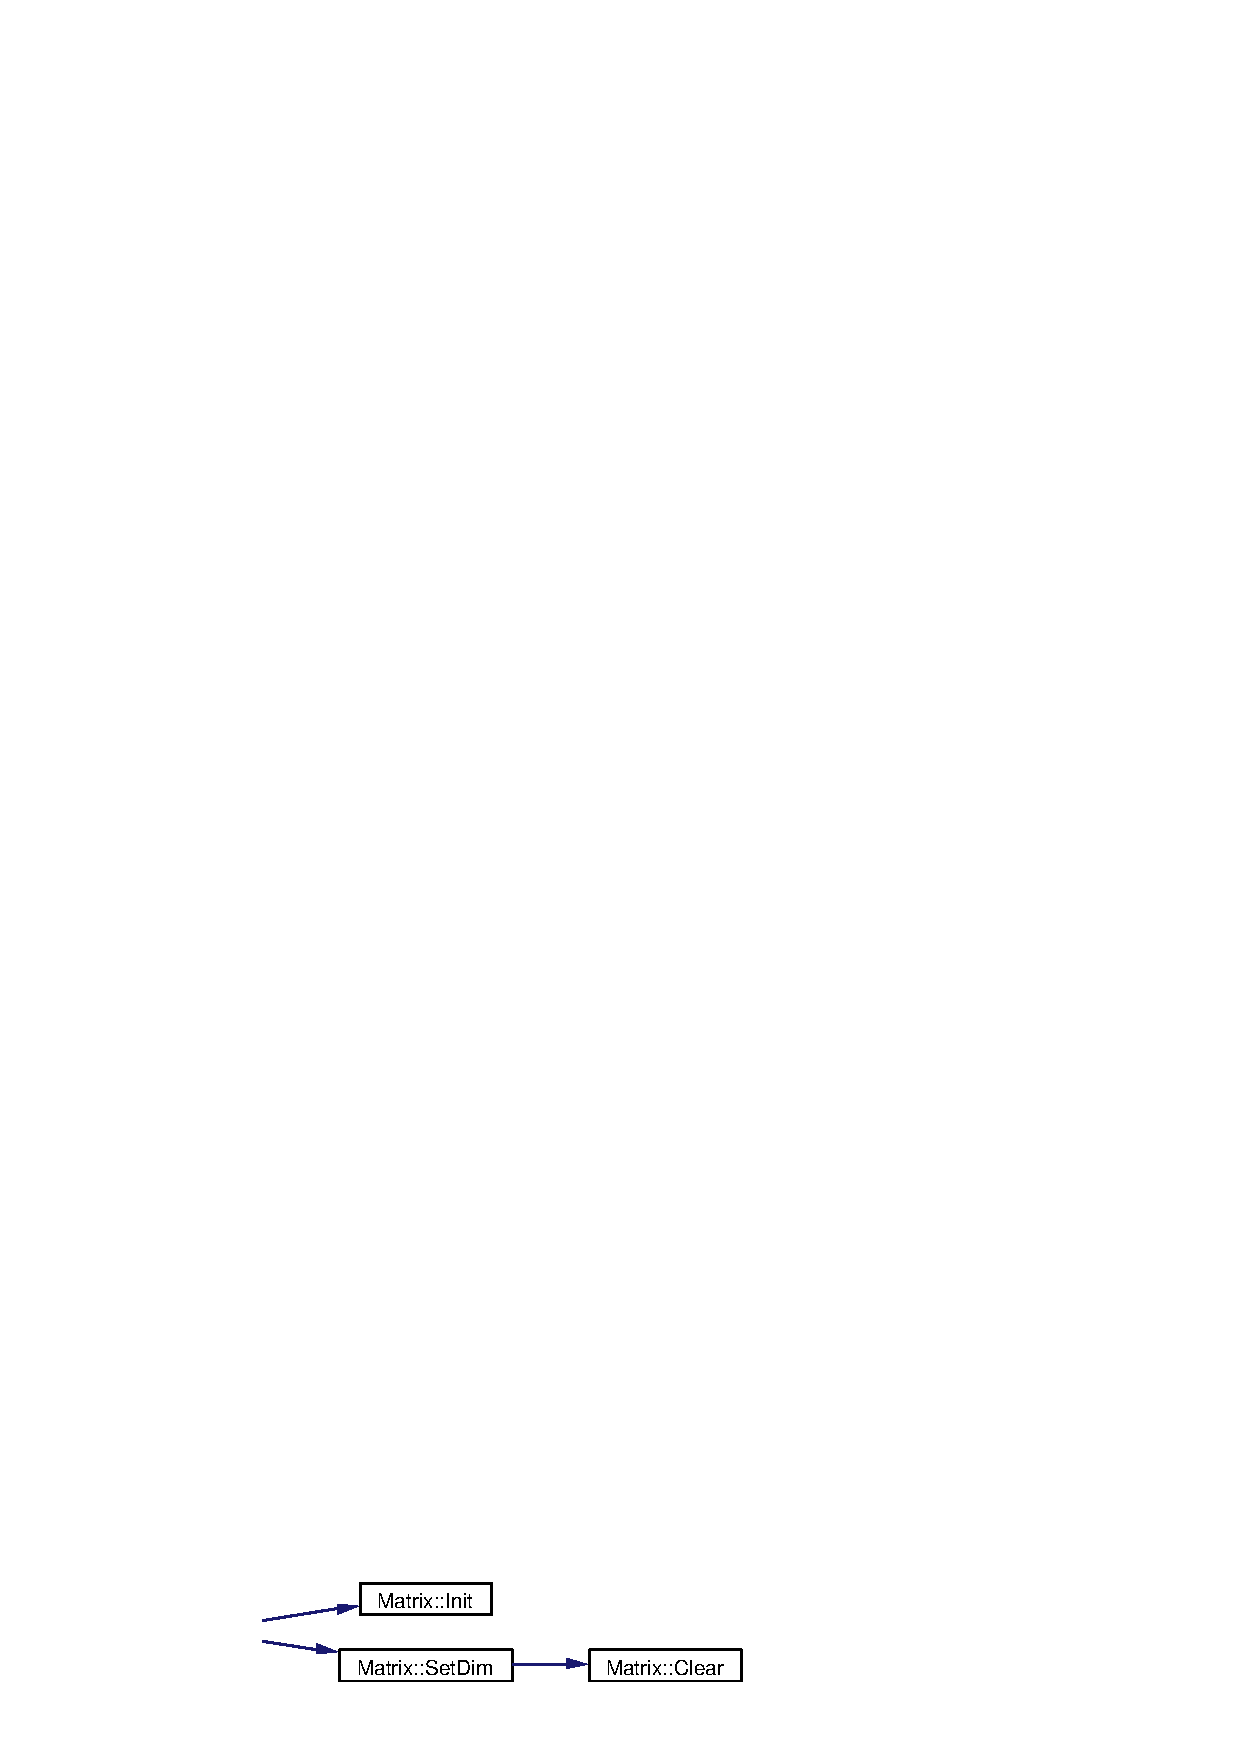
\includegraphics[width=182pt]{classMatrix_a0_cgraph}
\end{center}
\end{figure}
\index{Matrix@{Matrix}!Matrix@{Matrix}}
\index{Matrix@{Matrix}!Matrix@{Matrix}}
\subsubsection{\setlength{\rightskip}{0pt plus 5cm}Matrix::Matrix (const {\bf Matrix} \& {\em m})}\label{classMatrix_a1}


Matrix Copy Constructor 

Definition at line 74 of file matrix.cpp.

References \_\-vector, matrix, Set\-Dim(), x, and y.

Here is the call graph for this function:\begin{figure}[H]
\begin{center}
\leavevmode

\includegraphics[width=182pt]{classMatrix_a1_cgraph}
\end{center}
\end{figure}
\index{Matrix@{Matrix}!~Matrix@{$\sim$Matrix}}
\index{~Matrix@{$\sim$Matrix}!Matrix@{Matrix}}
\subsubsection{\setlength{\rightskip}{0pt plus 5cm}Matrix::$\sim${\bf Matrix} ()}\label{classMatrix_a2}


Destructor: Matrix 

Definition at line 95 of file matrix.cpp.

References Clear().

Here is the call graph for this function:\begin{figure}[H]
\begin{center}
\leavevmode
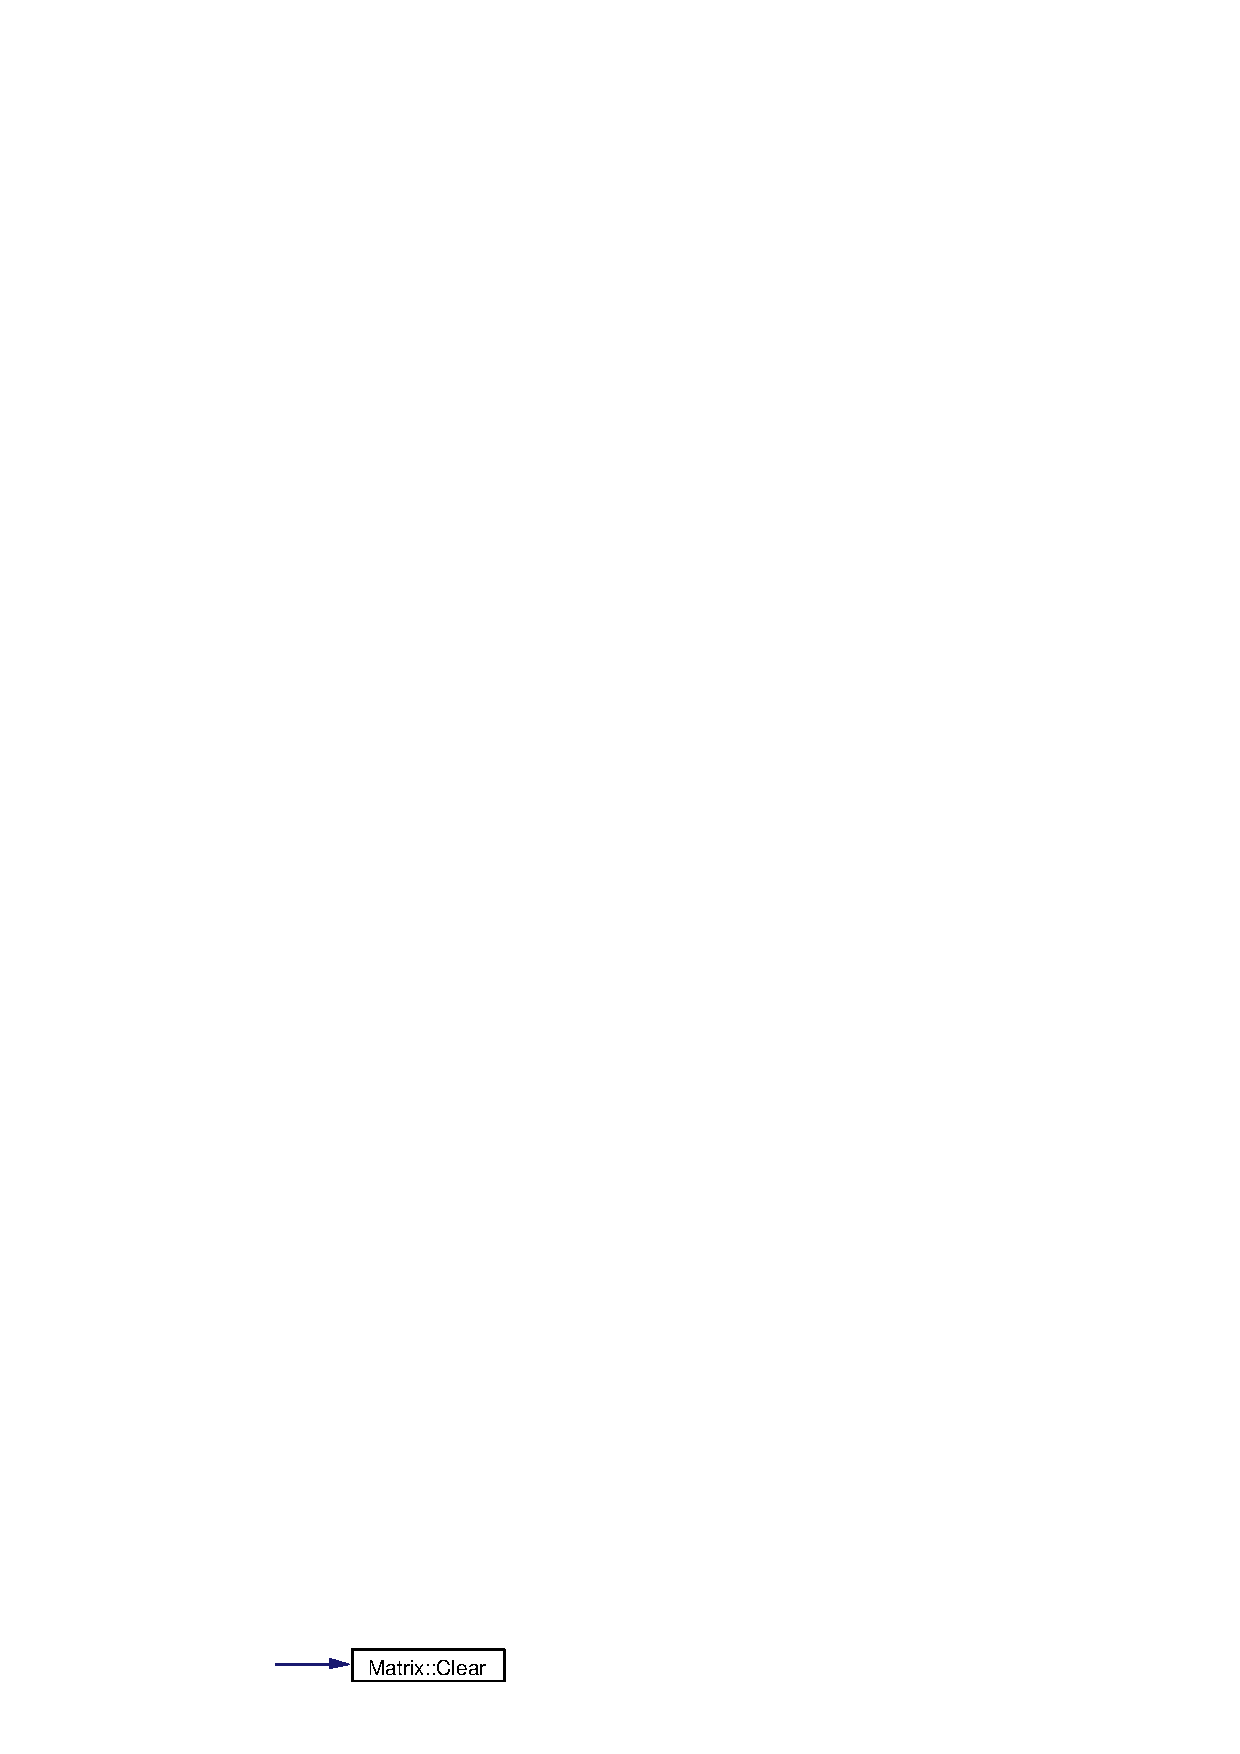
\includegraphics[width=125pt]{classMatrix_a2_cgraph}
\end{center}
\end{figure}


\subsection{Member Function Documentation}
\index{Matrix@{Matrix}!AdjustMatrix@{AdjustMatrix}}
\index{AdjustMatrix@{AdjustMatrix}!Matrix@{Matrix}}
\subsubsection{\setlength{\rightskip}{0pt plus 5cm}void Matrix::Adjust\-Matrix (int {\em type}, int {\em stime\-Matrix}, int {\em end\-Loc\-M}, int {\em slope}, int {\em from}, int {\em to})}\label{classMatrix_a10}


PUBLIC: ADJUSTMATRIX. Blocks the locations covered by the duration (dur\-Matrix). The edges are smoothed following a user define slope. 

Definition at line 297 of file matrix.cpp.

References matrix, Smooth(), and y.

Referenced by Event::Adjustments().

Here is the call graph for this function:\begin{figure}[H]
\begin{center}
\leavevmode
\includegraphics[width=144pt]{classMatrix_a10_cgraph}
\end{center}
\end{figure}
\index{Matrix@{Matrix}!AdjustVector@{AdjustVector}}
\index{AdjustVector@{AdjustVector}!Matrix@{Matrix}}
\subsubsection{\setlength{\rightskip}{0pt plus 5cm}void Matrix::Adjust\-Vector (int {\em type}, int {\em remain\-O}, int {\em from}, int {\em to})}\label{classMatrix_a9}


PUBLIC: ADJUSTVECTOR.

If remain\-O is -1, sets each element of the vector in the range specified by from and to to 0. If remain\-O is 0, sets the vector element specified by type to 0. Otherwise, decreases the vector element specified by type by 1/(remain0 + 1) for each element in the matrix line specified by type that is greater than 0. Finally, normalizes the vector element range specified by from and to. 

Definition at line 246 of file matrix.cpp.

References \_\-vector, matrix, sever, and y.

Referenced by Event::Adjustments().\index{Matrix@{Matrix}!BuildMatrix@{BuildMatrix}}
\index{BuildMatrix@{BuildMatrix}!Matrix@{Matrix}}
\subsubsection{\setlength{\rightskip}{0pt plus 5cm}void Matrix::Build\-Matrix (double {\em array}[$\,$])}\label{classMatrix_a11}


Build\-Matrix 

Definition at line 413 of file matrix.cpp.\index{Matrix@{Matrix}!BuildMatrix2@{BuildMatrix2}}
\index{BuildMatrix2@{BuildMatrix2}!Matrix@{Matrix}}
\subsubsection{\setlength{\rightskip}{0pt plus 5cm}void Matrix::Build\-Matrix2 ({\bf List}$<$ int $>$ \&, int)}\label{classMatrix_a12}


\index{Matrix@{Matrix}!ChooseM@{ChooseM}}
\index{ChooseM@{ChooseM}!Matrix@{Matrix}}
\subsubsection{\setlength{\rightskip}{0pt plus 5cm}void Matrix::Choose\-M (int \& {\em r}, int \& {\em c})}\label{classMatrix_a15}


Choose\-M

Same as Choose\-M but returns the values directly to the caller through the reference params r and c. 

Definition at line 462 of file matrix.cpp.

References Choose\-M(), col, and row.

Here is the call graph for this function:\begin{figure}[H]
\begin{center}
\leavevmode
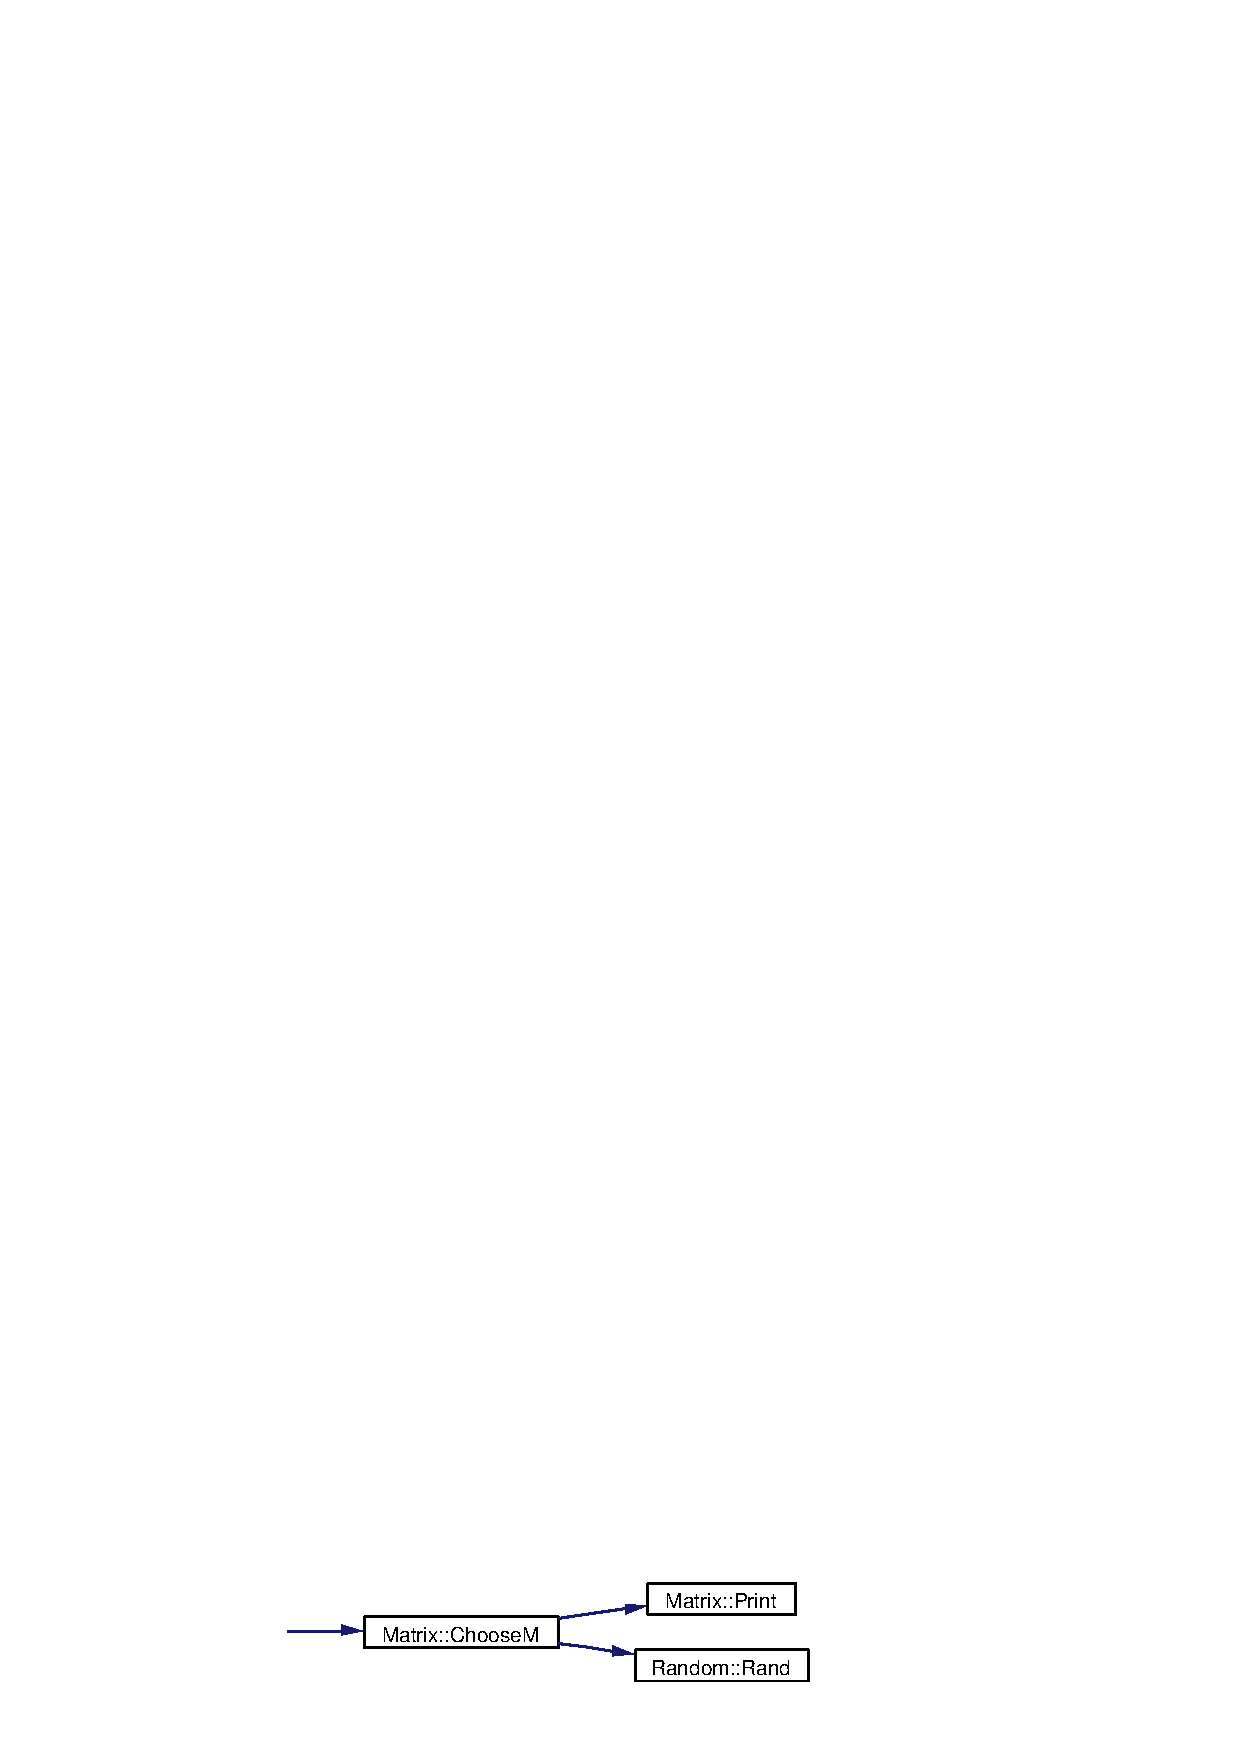
\includegraphics[width=198pt]{classMatrix_a15_cgraph}
\end{center}
\end{figure}
\index{Matrix@{Matrix}!ChooseM@{ChooseM}}
\index{ChooseM@{ChooseM}!Matrix@{Matrix}}
\subsubsection{\setlength{\rightskip}{0pt plus 5cm}void Matrix::Choose\-M ()}\label{classMatrix_a14}


STATIC PUBLIC: CHOOSEM

Chooses an element out of the probability matrix, based on each element's associated probability and a randomly generated number 

Definition at line 432 of file matrix.cpp.

References col, matrix, Print(), Random::Rand(), row, x, and y.

Referenced by Choose\-M(), Event::Find\-Dur(), and Event::Obj\-Coordinates().

Here is the call graph for this function:\begin{figure}[H]
\begin{center}
\leavevmode
\includegraphics[width=133pt]{classMatrix_a14_cgraph}
\end{center}
\end{figure}
\index{Matrix@{Matrix}!Clear@{Clear}}
\index{Clear@{Clear}!Matrix@{Matrix}}
\subsubsection{\setlength{\rightskip}{0pt plus 5cm}void Matrix::Clear ()}\label{classMatrix_a29}


PUBLIC: CLEAR. Deletes the matrix and sets its dimensions to 0. 

Definition at line 177 of file matrix.cpp.

References \_\-vector, matrix, x, and y.

Referenced by operator=(), Set\-Dim(), and $\sim$Matrix().\index{Matrix@{Matrix}!Envelopes@{Envelopes}}
\index{Envelopes@{Envelopes}!Matrix@{Matrix}}
\subsubsection{\setlength{\rightskip}{0pt plus 5cm}void Matrix::Envelopes (vector$<$ Collection$<$ xy\_\-point $>$ $>$ {\em xy\-Collection}, vector$<$ vector$<$ string $>$ $>$ {\em segment\-Types}, vector$<$ vector$<$ string $>$ $>$ {\em segment\-Fixed})}\label{classMatrix_a20}




Definition at line 576 of file matrix.cpp.

References matrix, x, and y.\index{Matrix@{Matrix}!Envelopes@{Envelopes}}
\index{Envelopes@{Envelopes}!Matrix@{Matrix}}
\subsubsection{\setlength{\rightskip}{0pt plus 5cm}void Matrix::Envelopes (char $\ast$ {\em file\-Name}, vector$<$ Collection$<$ xy\_\-point $>$ $>$ {\em xy\-Collection}, vector$<$ vector$<$ string $>$ $>$ {\em segment\-Types}, vector$<$ vector$<$ string $>$ $>$ {\em segment\-Fixed})}\label{classMatrix_a19}


\index{Matrix@{Matrix}!Envelopes@{Envelopes}}
\index{Envelopes@{Envelopes}!Matrix@{Matrix}}
\subsubsection{\setlength{\rightskip}{0pt plus 5cm}void Matrix::Envelopes (vector$<$ float $>$ {\em probs}, vector$<$ int $>$ {\em env\-Nums}, vector$<$ float $>$ {\em coeffs})}\label{classMatrix_a18}


\index{Matrix@{Matrix}!Envelopes@{Envelopes}}
\index{Envelopes@{Envelopes}!Matrix@{Matrix}}
\subsubsection{\setlength{\rightskip}{0pt plus 5cm}void Matrix::Envelopes (vector$<$ float $>$ {\em probs}, vector$<$ Envelope $\ast$ $>$ {\em env\-List})}\label{classMatrix_a17}


PUBLIC: Envelopes. Creates an envelope and loads envelopes from the library and finds their values corresponding to each sieve location (attack point). NB. we deal here with sieve locations and not with actual time values. 

Definition at line 557 of file matrix.cpp.

References matrix, x, and y.\index{Matrix@{Matrix}!Envelopes@{Envelopes}}
\index{Envelopes@{Envelopes}!Matrix@{Matrix}}
\subsubsection{\setlength{\rightskip}{0pt plus 5cm}void Matrix::Envelopes (char $\ast$ {\em file\-Name})}\label{classMatrix_a16}




Referenced by Event::New\-Create\-Matrices().\index{Matrix@{Matrix}!GetValueAt@{GetValueAt}}
\index{GetValueAt@{GetValueAt}!Matrix@{Matrix}}
\subsubsection{\setlength{\rightskip}{0pt plus 5cm}double Matrix::Get\-Value\-At (int {\em x}, int {\em y})}\label{classMatrix_a25}


\index{Matrix@{Matrix}!GetVector@{GetVector}}
\index{GetVector@{GetVector}!Matrix@{Matrix}}
\subsubsection{\setlength{\rightskip}{0pt plus 5cm}void Matrix::Get\-Vector (vector$<$ float $>$ {\em new\-Vector})}\label{classMatrix_a7}


PUBLIC: Get\-Vector. Read or Compute a vector from a file. 

Definition at line 647 of file matrix.cpp.

References \_\-vector, and x.\index{Matrix@{Matrix}!GetVector@{GetVector}}
\index{GetVector@{GetVector}!Matrix@{Matrix}}
\subsubsection{\setlength{\rightskip}{0pt plus 5cm}void Matrix::Get\-Vector (char $\ast$ {\em file\-Name})}\label{classMatrix_a6}


PUBLIC: Get\-Vector. Read or Compute a vector from a file. 

Referenced by Event::New\-Create\-Matrices().\index{Matrix@{Matrix}!GetX@{GetX}}
\index{GetX@{GetX}!Matrix@{Matrix}}
\subsubsection{\setlength{\rightskip}{0pt plus 5cm}int Matrix::Get\-X ()}\label{classMatrix_a30}


PUBLIC: Get\-X. Gets the value of the first subscript of the matrix. 

Definition at line 136 of file matrix.cpp.

References x.\index{Matrix@{Matrix}!GetY@{GetY}}
\index{GetY@{GetY}!Matrix@{Matrix}}
\subsubsection{\setlength{\rightskip}{0pt plus 5cm}int Matrix::Get\-Y ()}\label{classMatrix_a31}


PUBLIC: Get\-Y. Gets the value of the second subscript of the matrix. 

Definition at line 148 of file matrix.cpp.

References y.\index{Matrix@{Matrix}!IncludeArray@{IncludeArray}}
\index{IncludeArray@{IncludeArray}!Matrix@{Matrix}}
\subsubsection{\setlength{\rightskip}{0pt plus 5cm}void Matrix::Include\-Array (double {\em array}[$\,$], int {\em from}, int {\em to})}\label{classMatrix_a5}


Include\-Array. Multiplies the elements of an existing matrix with those of an array of doubles. Each matrix line between a lower limit (from) and an upper limit (to) is multiplied by the same array, each element of the array with an element of the matrix line. 

Definition at line 379 of file matrix.cpp.

References matrix, and y.

Referenced by Mult(), Event::New\-Create\-Matrices(), and Event::Obj\-Coordinates().\index{Matrix@{Matrix}!IncludeVector@{IncludeVector}}
\index{IncludeVector@{IncludeVector}!Matrix@{Matrix}}
\subsubsection{\setlength{\rightskip}{0pt plus 5cm}void Matrix::Include\-Vector ()}\label{classMatrix_a8}


Include\-Vector. Multiplies the elements of an existing matrix with those of avector of doubles. Each matrix line is multiplied by the same vector elemet, one vector element per line. 

Definition at line 397 of file matrix.cpp.

References \_\-vector, matrix, x, and y.\index{Matrix@{Matrix}!Init@{Init}}
\index{Init@{Init}!Matrix@{Matrix}}
\subsubsection{\setlength{\rightskip}{0pt plus 5cm}void Matrix::Init (double {\em init})}\label{classMatrix_a26}


PUBLIC: Init. Initialize the matrix with the same value (usually 0) 

Definition at line 160 of file matrix.cpp.

References matrix, x, and y.

Referenced by Matrix().\index{Matrix@{Matrix}!Interpol@{Interpol}}
\index{Interpol@{Interpol}!Matrix@{Matrix}}
\subsubsection{\setlength{\rightskip}{0pt plus 5cm}void Matrix::Interpol (int {\em array\-Size}, double {\em array}[$\,$])}\label{classMatrix_a21}


PUBLIC: INTERPOL. Given the values for a few points interpolates the values for the rest of the array 

Definition at line 757 of file matrix.cpp.

References y.

Referenced by Mult().\index{Matrix@{Matrix}!Mult@{Mult}}
\index{Mult@{Mult}!Matrix@{Matrix}}
\subsubsection{\setlength{\rightskip}{0pt plus 5cm}void Matrix::Mult (int {\em remain\-O}, float {\em density}, int {\em type}, int {\em dur\-Loc}, int {\em dur\-Array}[$\,$], int {\em stime\-Matrix}, int {\em star\-Tarray}[$\,$])}\label{classMatrix_a22}


MULT. Finds the most desirable duration given the density and the number of unassigned yet objects. Creates an array centered around this \char`\"{}peak\char`\"{} then multiplies the line of the existing duration matrix which corresponds to the type already chosen with the array. 

Definition at line 699 of file matrix.cpp.

References Include\-Array(), Interpol(), and y.

Referenced by Event::Find\-Dur().

Here is the call graph for this function:\begin{figure}[H]
\begin{center}
\leavevmode
\includegraphics[width=137pt]{classMatrix_a22_cgraph}
\end{center}
\end{figure}
\index{Matrix@{Matrix}!Normalize@{Normalize}}
\index{Normalize@{Normalize}!Matrix@{Matrix}}
\subsubsection{\setlength{\rightskip}{0pt plus 5cm}void Matrix::Normalize ()}\label{classMatrix_a23}


Normalize. Takes a two-dimenssional array of doubles, divides each element by the sum of all elements, and adds the value to the preceding value (sum of values) so that the last element is always 1. 

Definition at line 792 of file matrix.cpp.

References matrix, x, and y.

Referenced by Event::Find\-Dur().\index{Matrix@{Matrix}!operator()@{operator()}}
\index{operator()@{operator()}!Matrix@{Matrix}}
\subsubsection{\setlength{\rightskip}{0pt plus 5cm}double Matrix::operator() (int {\em a}, int {\em b})}\label{classMatrix_a4}




Definition at line 100 of file matrix.cpp.

References matrix.\index{Matrix@{Matrix}!operator=@{operator=}}
\index{operator=@{operator=}!Matrix@{Matrix}}
\subsubsection{\setlength{\rightskip}{0pt plus 5cm}{\bf Matrix} \& Matrix::operator= ({\bf Matrix} \& {\em m})}\label{classMatrix_a3}


PUBLIC: OPERATOR=. 

Definition at line 199 of file matrix.cpp.

References \_\-vector, Clear(), matrix, Set\-Dim(), x, and y.

Here is the call graph for this function:\begin{figure}[H]
\begin{center}
\leavevmode
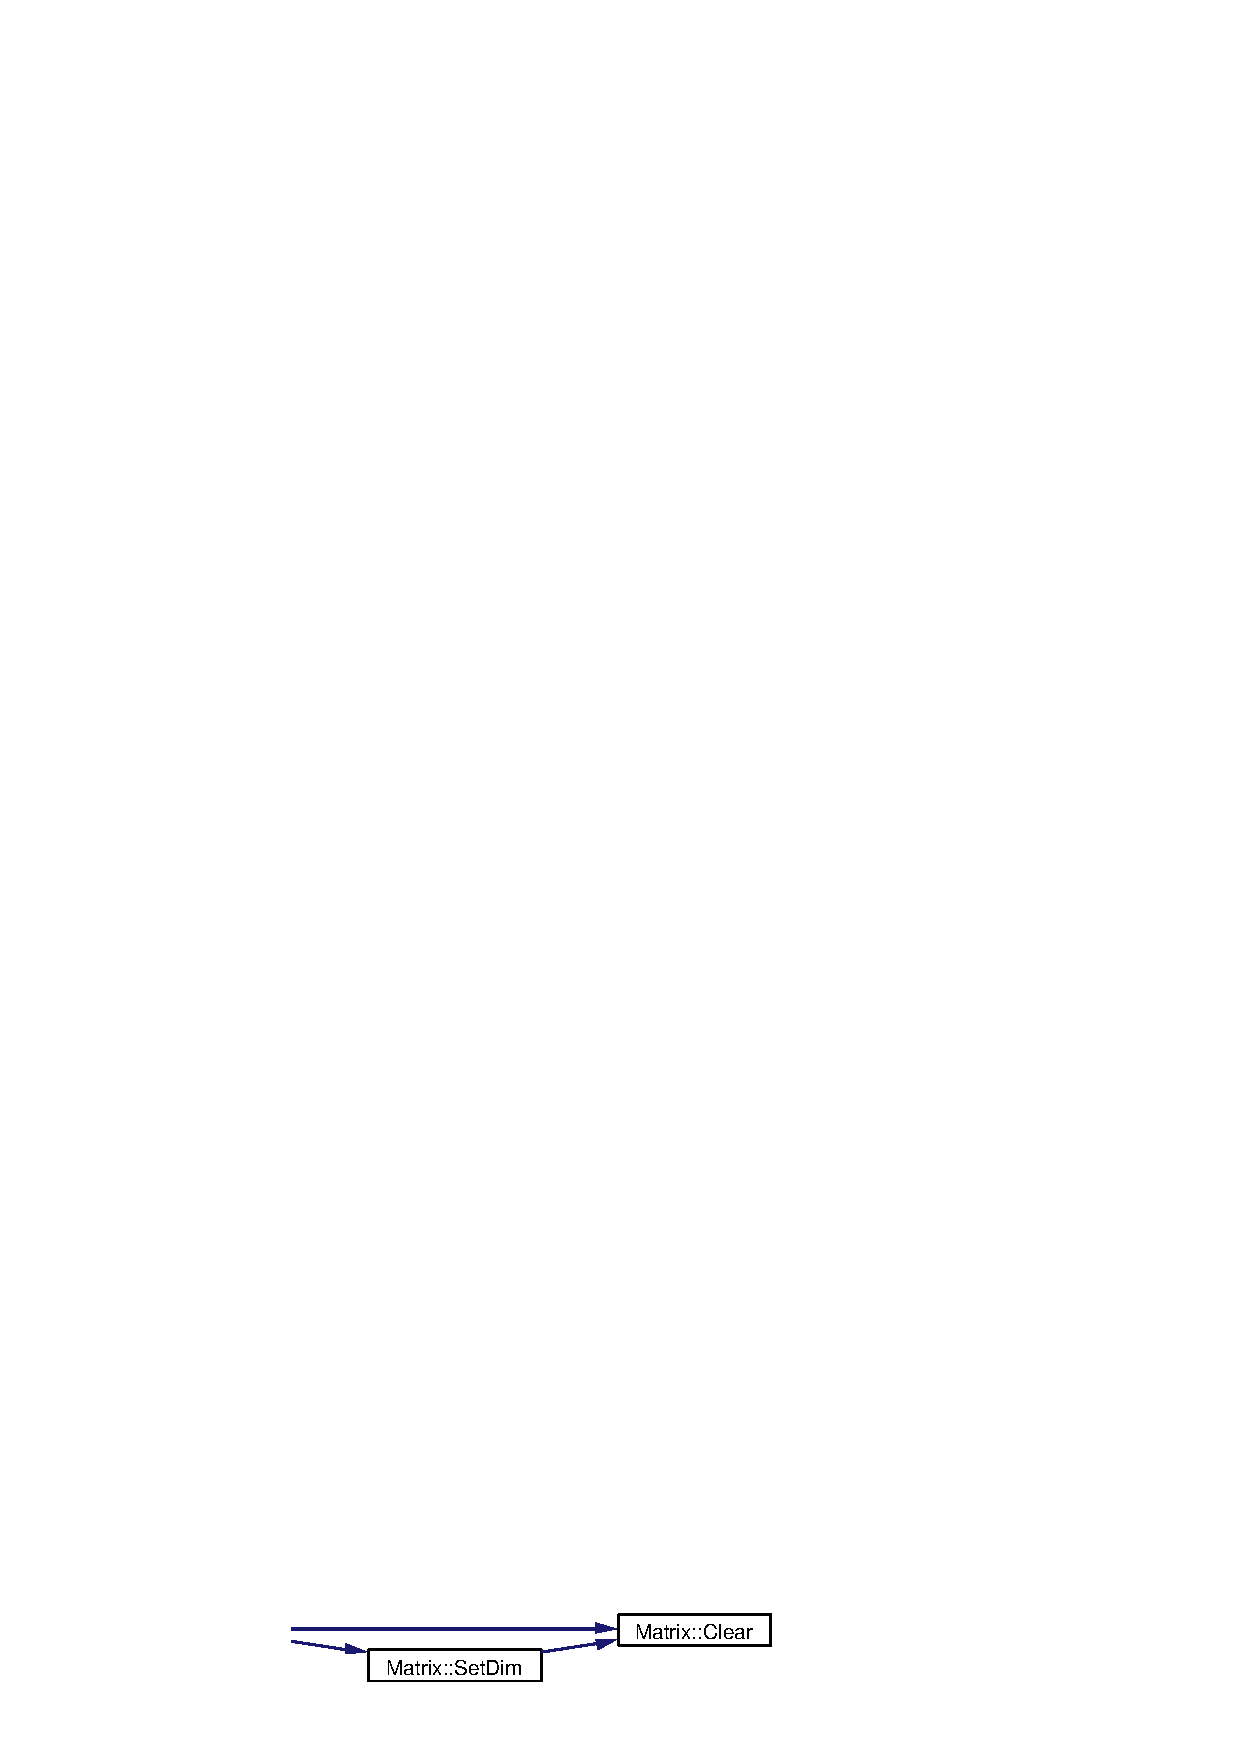
\includegraphics[width=189pt]{classMatrix_a3_cgraph}
\end{center}
\end{figure}
\index{Matrix@{Matrix}!Print@{Print}}
\index{Print@{Print}!Matrix@{Matrix}}
\subsubsection{\setlength{\rightskip}{0pt plus 5cm}void Matrix::Print ()}\label{classMatrix_a27}


Print. Prints all the elements of the matrix. Useful in testing. 

Definition at line 825 of file matrix.cpp.

References matrix, x, and y.

Referenced by Choose\-M(), and Event::Obj\-Coordinates().\index{Matrix@{Matrix}!PrintVector@{PrintVector}}
\index{PrintVector@{PrintVector}!Matrix@{Matrix}}
\subsubsection{\setlength{\rightskip}{0pt plus 5cm}void Matrix::Print\-Vector ()}\label{classMatrix_a28}


Print\-Vectors. Prints a vector/array on a 8 column format. 

Definition at line 845 of file matrix.cpp.

References \_\-vector, and x.

Referenced by Event::Obj\-Coordinates().\index{Matrix@{Matrix}!SetDim@{SetDim}}
\index{SetDim@{SetDim}!Matrix@{Matrix}}
\subsubsection{\setlength{\rightskip}{0pt plus 5cm}void Matrix::Set\-Dim (int {\em x}, int {\em y})}\label{classMatrix_a24}


PUBLIC: Set\-Dim Sets the dimensions of the matrix, vector, and the probability array. 

Definition at line 112 of file matrix.cpp.

References \_\-vector, Clear(), and matrix.

Referenced by Matrix(), and operator=().

Here is the call graph for this function:\begin{figure}[H]
\begin{center}
\leavevmode
\includegraphics[width=123pt]{classMatrix_a24_cgraph}
\end{center}
\end{figure}
\index{Matrix@{Matrix}!Smooth@{Smooth}}
\index{Smooth@{Smooth}!Matrix@{Matrix}}
\subsubsection{\setlength{\rightskip}{0pt plus 5cm}void Matrix::Smooth (int {\em line}, int {\em slope}, int {\em start}, int {\em finish}, int {\em flag})\hspace{0.3cm}{\tt  [private]}}\label{classMatrix_d0}


PRIVATE: SMOOTH

If flag is 1, smooths the the matrix locations leading up to or trailing away from a sound. 

Definition at line 330 of file matrix.cpp.

References matrix, and y.

Referenced by Adjust\-Matrix().\index{Matrix@{Matrix}!TrimMatrix@{TrimMatrix}}
\index{TrimMatrix@{TrimMatrix}!Matrix@{Matrix}}
\subsubsection{\setlength{\rightskip}{0pt plus 5cm}void Matrix::Trim\-Matrix (int {\em type}, float {\em density}, int {\em remain\-O}, int {\em dur\-Loc})}\label{classMatrix_a13}


TRIMMATRIX. Reads in individual arrays, builds another array(s) and multiplies it/them with the first set in order to obtain a weighted mean. Resulting matrix is normalized/scaled. $\ast$$\ast$This function is used only for the duration matrix and performs similar tasks as the Build\-Matrix function used only for the type/attacks matrix.$\ast$$\ast$ 

Definition at line 664 of file matrix.cpp.

References matrix, x, and y.

Referenced by Event::Find\-Dur().

\subsection{Friends And Related Function Documentation}
\index{Matrix@{Matrix}!Event@{Event}}
\index{Event@{Event}!Matrix@{Matrix}}
\subsubsection{\setlength{\rightskip}{0pt plus 5cm}friend class {\bf Event}\hspace{0.3cm}{\tt  [friend]}}\label{classMatrix_n0}




Definition at line 127 of file matrix.h.\index{Matrix@{Matrix}!operator<<@{operator$<$$<$}}
\index{operator<<@{operator$<$$<$}!Matrix@{Matrix}}
\subsubsection{\setlength{\rightskip}{0pt plus 5cm}ostream\& operator$<$$<$ (ostream \& {\em s}, {\bf Matrix} \& {\em m})\hspace{0.3cm}{\tt  [friend]}}\label{classMatrix_n1}


PUBLIC: OPERATOR$<$$<$. 

Definition at line 220 of file matrix.cpp.

\subsection{Member Data Documentation}
\index{Matrix@{Matrix}!_vector@{\_\-vector}}
\index{_vector@{\_\-vector}!Matrix@{Matrix}}
\subsubsection{\setlength{\rightskip}{0pt plus 5cm}double$\ast$ {\bf Matrix::\_\-vector}\hspace{0.3cm}{\tt  [private]}}\label{classMatrix_r4}




Definition at line 138 of file matrix.h.

Referenced by Adjust\-Vector(), Clear(), Get\-Vector(), Include\-Vector(), Matrix(), operator=(), Print\-Vector(), and Set\-Dim().\index{Matrix@{Matrix}!col@{col}}
\index{col@{col}!Matrix@{Matrix}}
\subsubsection{\setlength{\rightskip}{0pt plus 5cm}int {\bf Matrix::col}}\label{classMatrix_o0}




Definition at line 129 of file matrix.h.

Referenced by Choose\-M(), and Event::Obj\-Coordinates().\index{Matrix@{Matrix}!matrix@{matrix}}
\index{matrix@{matrix}!Matrix@{Matrix}}
\subsubsection{\setlength{\rightskip}{0pt plus 5cm}double$\ast$$\ast$ {\bf Matrix::matrix}}\label{classMatrix_o2}




Definition at line 130 of file matrix.h.

Referenced by Adjust\-Matrix(), Adjust\-Vector(), Choose\-M(), Clear(), Envelopes(), Event::Find\-Len(), Include\-Array(), Include\-Vector(), Init(), Matrix(), Normalize(), operator()(), operator$<$$<$(), operator=(), Print(), Set\-Dim(), Smooth(), and Trim\-Matrix().\index{Matrix@{Matrix}!row@{row}}
\index{row@{row}!Matrix@{Matrix}}
\subsubsection{\setlength{\rightskip}{0pt plus 5cm}int {\bf Matrix::row}}\label{classMatrix_o1}




Definition at line 129 of file matrix.h.

Referenced by Choose\-M(), Event::Find\-Dur(), and Event::Obj\-Coordinates().\index{Matrix@{Matrix}!sever@{sever}}
\index{sever@{sever}!Matrix@{Matrix}}
\subsubsection{\setlength{\rightskip}{0pt plus 5cm}int {\bf Matrix::sever}\hspace{0.3cm}{\tt  [private]}}\label{classMatrix_r1}




Definition at line 136 of file matrix.h.

Referenced by Adjust\-Vector().\index{Matrix@{Matrix}!stProb@{stProb}}
\index{stProb@{stProb}!Matrix@{Matrix}}
\subsubsection{\setlength{\rightskip}{0pt plus 5cm}double$\ast$ {\bf Matrix::st\-Prob}\hspace{0.3cm}{\tt  [private]}}\label{classMatrix_r0}




Definition at line 134 of file matrix.h.\index{Matrix@{Matrix}!x@{x}}
\index{x@{x}!Matrix@{Matrix}}
\subsubsection{\setlength{\rightskip}{0pt plus 5cm}int {\bf Matrix::x}\hspace{0.3cm}{\tt  [private]}}\label{classMatrix_r2}




Definition at line 137 of file matrix.h.

Referenced by Choose\-M(), Clear(), Envelopes(), Get\-Vector(), Get\-X(), Include\-Vector(), Init(), Matrix(), Normalize(), operator$<$$<$(), operator=(), Print(), Print\-Vector(), and Trim\-Matrix().\index{Matrix@{Matrix}!y@{y}}
\index{y@{y}!Matrix@{Matrix}}
\subsubsection{\setlength{\rightskip}{0pt plus 5cm}int {\bf Matrix::y}\hspace{0.3cm}{\tt  [private]}}\label{classMatrix_r3}




Definition at line 137 of file matrix.h.

Referenced by Adjust\-Matrix(), Adjust\-Vector(), Choose\-M(), Clear(), Envelopes(), Get\-Y(), Include\-Array(), Include\-Vector(), Init(), Interpol(), Matrix(), Mult(), Normalize(), operator$<$$<$(), operator=(), Print(), Smooth(), and Trim\-Matrix().

The documentation for this class was generated from the following files:\begin{CompactItemize}
\item 
{\bf matrix.h}\item 
{\bf matrix.cpp}\end{CompactItemize}
